\chapter{روش پیشنهادی و نتیجه‌گیری}
\label{ch:method}
\section{مقدمه}
در فصل‌های پیشین، مسئله تولید توضیحات شطرنجی و ضرورت تفکیک روانی متن از صحت محتوای آن مطرح شد. در این فصل، روش پیاده‌سازی سامانه «نگهبان خطا» و فرایند ارزیابی آن تشریح می‌شود. ایده اصلی آن است که تحلیل موقعیت به موتور شطرنج سپرده شود و مدل زبانی، با دریافت شواهد تحلیلی و تغییرات صفحه، دلیل مناسب یا نامناسب بودن یک حرکت را به زبان قابل فهم بیان کند. به این ترتیب، سامانه علاوه بر تولید توضیح، بستری برای مقایسه مدل‌های مختلف بر روی ورودی‌های مشترک فراهم می‌کند.

ابتدا اجزای نرم‌افزار و نحوه انتقال اطلاعات میان آن‌ها معرفی می‌شود. سپس ساخت مجموعه آزمون، تولید پاسخ‌ها و معیارهای داوری توضیح داده می‌شوند. در ادامه، نتایج ثبت‌شده برای ۱۱ مدل بر روی ۶۰ نمونه تحلیل می‌شود و در پایان، دستاوردها، محدودیت‌ها و مسیرهای بهبود پروژه بیان می‌گردد. اعداد این فصل از پرونده‌های خروجی ارزیابی پروژه استخراج شده‌اند و نمودارها نیز بر مبنای همان داده‌ها ترسیم شده‌اند.

\section{طراحی و پیاده‌سازی روش پیشنهادی}
\subsection{معماری سامانه و جریان پردازش}
سامانه از سه بخش اصلی تشکیل شده است: رابط کاربری، بخش تحلیل شطرنج و بخش تولید توضیح. رابط کاربری با \lr{React} پیاده‌سازی شده و امکان نمایش صفحه و متن تحلیل را فراهم می‌کند. بخش پشتی با \lr{Python} و \lr{Flask} درخواست‌ها را پردازش کرده و ارتباط با موتور شطرنج و مدل زبانی را بر عهده دارد. مدل محلی از طریق \lr{llama.cpp}~\cite{llamacpp-doc} اجرا می‌شود؛ در مسیر آزمایش مدل‌ها نیز امکان استفاده از سرویس‌های سازگار با رابط برنامه‌نویسی مورد استفاده پروژه وجود دارد.

ورودی تحلیلی شامل وضعیت قبل و بعد از حرکت است. پس از تحلیل هر دو وضعیت با \lr{Stockfish}~\cite{stockfish-doc}، ویژگی‌های مهم صفحه استخراج و در یک پیام ساختاریافته قرار داده می‌شوند. مدل زبانی این پیام را دریافت کرده و توضیح نهایی را تولید می‌کند. در مسیر ارزیابی، پاسخ تولیدشده به همراه شناسه نمونه و نام مدل ذخیره می‌شود تا در مرحله بعد با توضیح مرجع همان نمونه مقایسه شود. شکل~\ref{fig:pipeline} این دو مسیر مرتبط را نشان می‌دهد.

\begin{figure}[htbp]
\centering
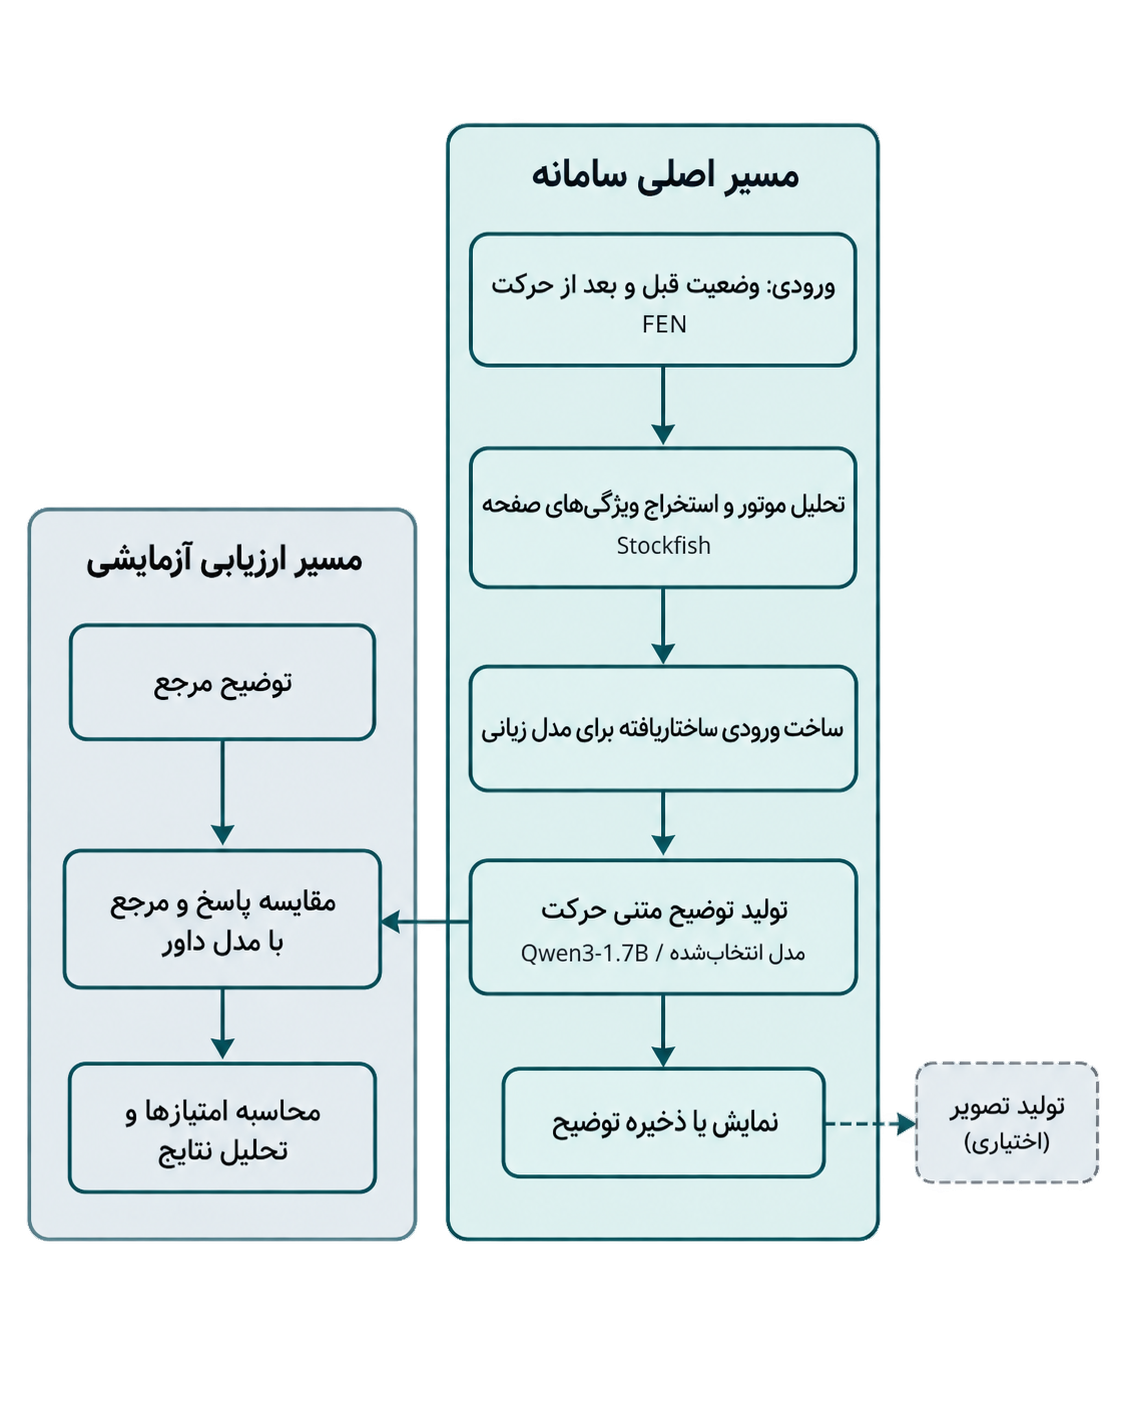
\includegraphics[width=0.93\linewidth]{chapter3_assets/pipeline_v2.png}
\caption{جریان پردازش و ارزیابی در سامانه پیشنهادی}
\label{fig:pipeline}
\end{figure}

\subsection{تحلیل موقعیت و استخراج ویژگی‌ها}
برای نمایش وضعیت صفحه از قالب \lr{FEN} استفاده می‌شود. این قالب علاوه بر محل مهره‌ها، اطلاعاتی مانند نوبت حرکت و حق قلعه‌رفتن را در اختیار بخش پردازش قرار می‌دهد. در پیاده‌سازی موجود، موتور با عمق جست‌وجوی ۱۷ فراخوانی می‌شود و تا سه ادامه پیشنهادی را بررسی می‌کند. تحلیل قبل و بعد از حرکت، شامل ارزیابی عددی و ادامه‌های پیشنهادی، بخشی از زمینه ورودی مدل زبانی را تشکیل می‌دهد. جهت ارزیابی باید ثابت بماند؛ در خروجی‌های ثبت‌شده، ارزیابی‌ها از دید سفید گزارش شده‌اند.

ماژول استخراج ویژگی‌ها برای هر دو رنگ اجرا می‌شود و تغییراتی مانند وجود مهره بدون دفاع، کاهش امنیت شاه، از دست رفتن کنترل مرکز، تأخیر در گسترش مهره‌ها و ضعف‌های ساختار پیاده‌ای را بررسی می‌کند. هدف این مرحله، برجسته‌کردن اطلاعاتی است که بیان آموزشی حرکت را آسان‌تر می‌سازند. این ویژگی‌ها حاصل قواعد پیاده‌سازی‌شده هستند و پوشش کامل تمام مفاهیم تاکتیکی و راهبردی شطرنج را تضمین نمی‌کنند. بنابراین، کنار هم قرار گرفتن ویژگی‌ها و تحلیل موتور به معنای تضمین صحت متن نهایی نیست؛ همین موضوع ضرورت ارزیابی مستقل خروجی را توضیح می‌دهد.

\subsection{ساخت ورودی و تولید توضیح}
در الگوی ورودی، از مدل خواسته می‌شود مانند یک مربی شطرنج، دلیل بهتر یا بدتر شدن موقعیت را در دو یا سه جمله کوتاه توضیح دهد. دستورها بر زبان ساده، بیان ایده به جای محاسبه و خودداری از تکرار نام حرکت‌ها، اعداد ارزیابی و خطوط موتور تأکید دارند. در نتیجه، میان «اطلاعاتی که مدل برای درک موقعیت دریافت می‌کند» و «اطلاعاتی که باید در متن آموزشی بازگو شود» تفاوت وجود دارد. مدل به شواهد عددی دسترسی دارد، اما باید پیامد آموزشی آن‌ها را بیان کند.

در کد پروژه دو روش تک‌مرحله‌ای و زنجیره‌ای پیش‌بینی شده است. روش تک‌مرحله‌ای مستقیماً از اطلاعات دو موقعیت و ویژگی‌های استخراج‌شده توضیح می‌سازد. در روش زنجیره‌ای، ابتدا برای موقعیت قبل و بعد توصیف جداگانه تولید می‌شود و سپس این توصیف‌ها در مرحله نهایی ترکیب می‌شوند. وجود این دو مسیر یک قابلیت نرم‌افزاری است؛ نتایج گزارش‌شده در این فصل، مقایسه کنترل‌شده این دو روش نیست و از آن‌ها نمی‌توان برتری یکی را نتیجه گرفت. مبنای مقایسه عددی، پاسخ‌های ذخیره‌شده مدل‌ها برای مجموعه مشترک آزمون است.

\subsection{مدل محلی و رابط کاربری}
در کنار مدل‌های عمومی، مدل کوچک اختصاصی با شناسه \lr{chess-q8\_0} ارزیابی شده است. مطابق دفترچه آموزش پروژه، مدل پایه \lr{Qwen3-1.7B} با \lr{۱٫۷} میلیارد پارامتر است و با روش \lr{LoRA} بر متن کتاب‌های شطرنج سازگار شده است. نسخه آزموده‌شده با کمی‌سازی \lr{Q8\_0} از طریق \lr{llama.cpp} به صورت محلی اجرا می‌شود. آموزش روی متن کتاب با آموزش نظارت‌شده بر جفت‌های «موقعیت و توضیح صحیح همان موقعیت» یکسان نیست؛ ازاین‌رو، آشنایی با ادبیات شطرنج لزوماً به اتصال درست متن به وضعیت صفحه منجر نمی‌شود. اندازه کوچک این مدل، مقایسه کیفیت آن با نسخه‌های بزرگ‌تر را به یکی از جنبه‌های مهم این آزمایش تبدیل می‌کند.

شکل~\ref{fig:ui} تصویر موجود در مستندات پروژه از رابط کاربری را نشان می‌دهد. صفحه شطرنج و بخش توضیح در کنار هم قرار گرفته‌اند تا کاربر بتواند متن را همراه وضعیت بازی مشاهده کند. این تصویر برای معرفی شکل ارائه خروجی استفاده شده است و نمونه‌ای از اثبات صحت تحلیل یا بخشی از نتایج کمی آزمون محسوب نمی‌شود.

\begin{figure}[htbp]
\centering
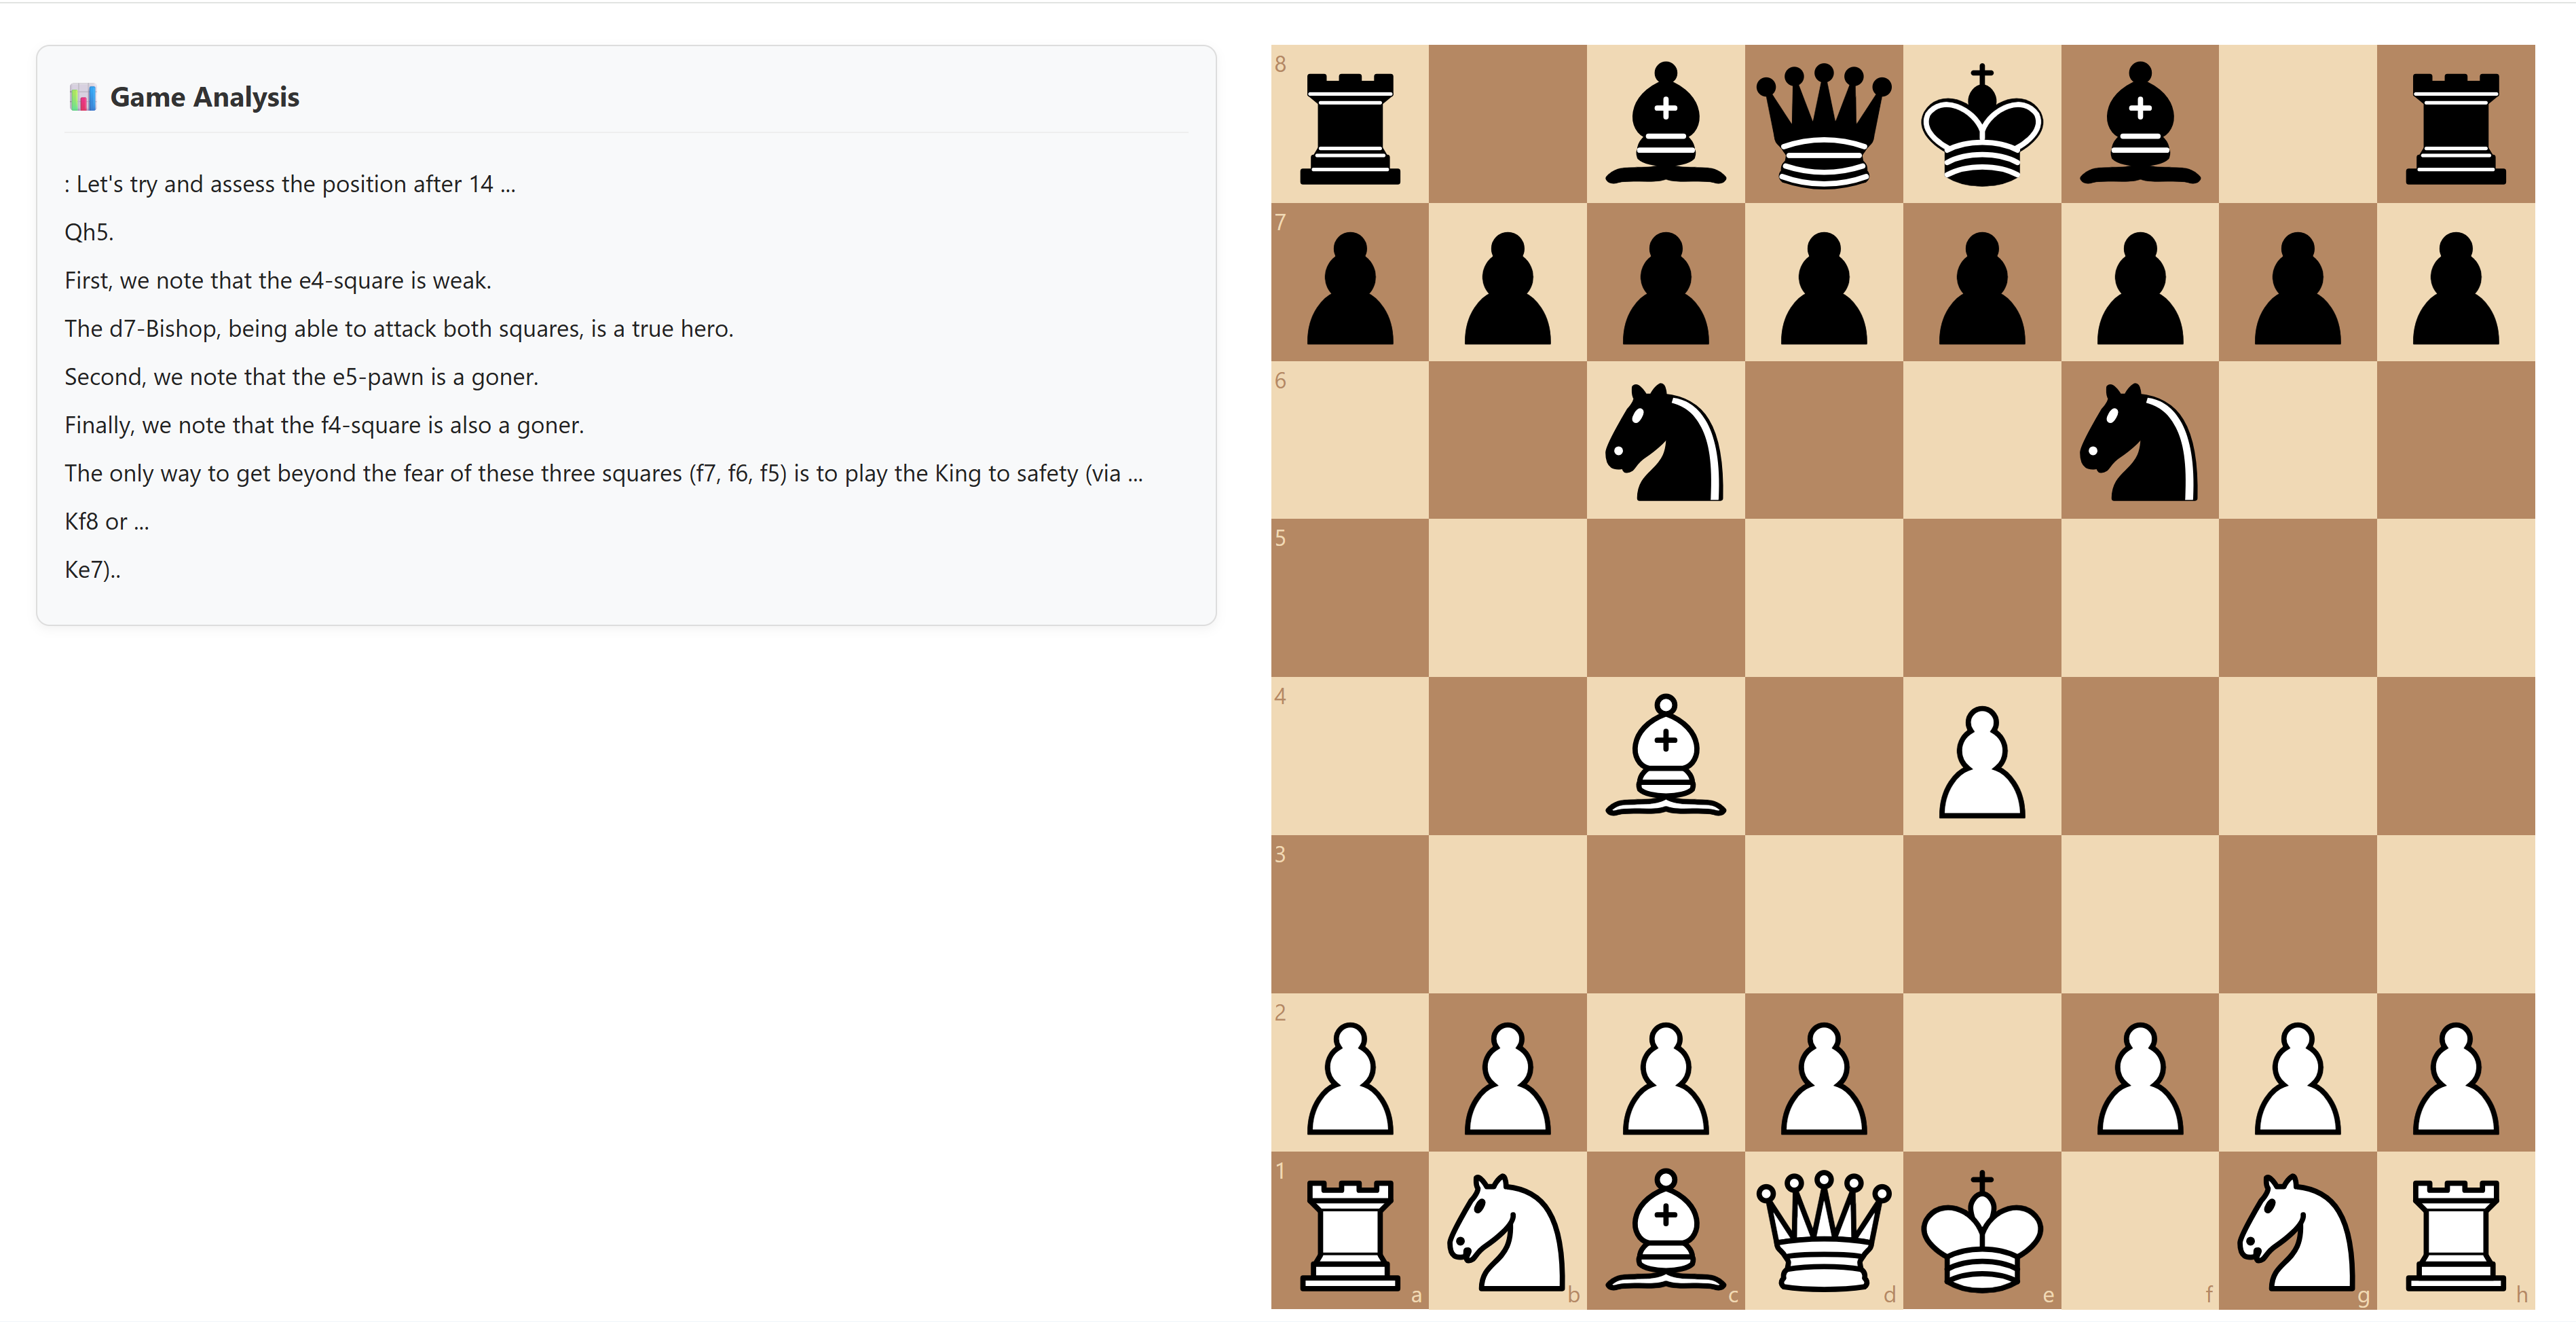
\includegraphics[width=\linewidth]{software_screenshot.png}
\caption{تصویر رابط کاربری ثبت‌شده در مستندات پروژه}
\label{fig:ui}
\end{figure}

\section{روش ارزیابی آزمایشی}
\subsection{تهیه و ساختار مجموعه آزمون}
مجموعه نهایی ارزیابی در پرونده \lr{evaluation\_dataset.tsv} شامل ۶۰ نمونه است. هر نمونه یک انتقال از وضعیت قبل به وضعیت بعد از حرکت را توصیف می‌کند. مجموعه به صورت متوازن از سه گروه مبتدی، متوسط و پیشرفته تشکیل شده و در هر گروه ۲۰ نمونه وجود دارد. همان‌طور که در فصل اول بیان شد، نمونه‌ها و توضیحات مرجع به صورت دستی بررسی و برچسب‌گذاری شده‌اند.

در اسکریپت دسته‌بندی بازی‌ها، میانگین امتیاز دو بازیکن مبنای گروه‌بندی است: کمتر از ۱۲۰۰ برای مبتدی، از ۱۲۰۰ تا کمتر از ۱۸۰۰ برای متوسط و ۱۸۰۰ و بالاتر برای پیشرفته. بازی‌های کوتاه‌تر از ۳۰ نیم‌حرکت کنار گذاشته می‌شوند. باید توجه داشت که سطح بازیکنان فقط مبنای دسته‌بندی منبع نمونه‌هاست و اندازه‌گیری مستقلی از دشواری تاکتیکی تک‌تک موقعیت‌ها نیست. همچنین تعداد بازی‌های اولیه با تعداد نمونه‌های نهایی آزمون تفاوت دارد؛ واحد محاسبه امتیاز در این فصل، یک موقعیت‌ـ‌حرکت است.

\begin{table}[htbp]
\centering
\caption{ترکیب مجموعه آزمون نهایی}
\label{tab:dataset}
\begin{tabular}{lrrr}
\toprule
گروه & تعداد نمونه & سهم از مجموعه & میانگین امتیاز بازیکنان در دسته‌بندی \\
\midrule
مبتدی & ۲۰ & \lr{۳۳٫۳} درصد & کمتر از ۱۲۰۰ \\
متوسط & ۲۰ & \lr{۳۳٫۳} درصد & ۱۲۰۰ تا کمتر از ۱۸۰۰ \\
پیشرفته & ۲۰ & \lr{۳۳٫۳} درصد & ۱۸۰۰ و بیشتر \\
\midrule
مجموع & ۶۰ & ۱۰۰ درصد & \lr{---} \\
\bottomrule
\end{tabular}
\end{table}

برای هر نمونه، شناسه، وضعیت قبل و بعد، حرکت، ورودی مدل، توضیح مرجع و گروه سطح ذخیره شده است. پاسخ‌های تولیدی نیز در پرونده‌های جداگانه با نام مدل نگهداری می‌شوند. در مرحله داوری، کلید ترکیبی «گروه و شناسه نمونه» برای تطبیق پاسخ و مرجع به کار می‌رود. این انتخاب اهمیت دارد، زیرا شناسه محلی یک حرکت ممکن است در گروه دیگری تکرار شود و تطبیق صرفاً بر اساس ترتیب سطرها یا شناسه تنها، قابل اتکا نیست.

\subsection{مدل‌های مقایسه‌شده و محدوده آزمایش}
در این ارزیابی، ۱۱ مدل پاسخ‌دهنده بررسی شده‌اند. شناسه‌های ثبت‌شده شامل مدل اختصاصی \lr{chess-q8\_0} و مدل‌های \lr{Llama-3.2-3B-Instruct-Q4\_K\_M}، \lr{gemma-3-12b-it-Q4\_0}، \lr{qwen3-30b-a3b}، \lr{gpt-oss-120b}، \lr{cf.llama-3.3-70b-instruct-fp8-fast}، \lr{cf.gemma-4-26b-a4b-it}، \lr{grok-4.3}، \lr{gemini-3.5-flash}، \lr{qwen3.7-plus} و \lr{gpt-5.5} هستند. نام‌های کوتاه‌تر در نمودارها و جدول نتایج به همین شناسه‌ها اشاره دارند و ادعایی درباره مشخصات منتشرنشده مدل‌ها ندارند.

هر مدل ۶۰ پاسخ در فایل ارزیابی دارد؛ بنابراین تحلیل اصلی بر ۶۶۰ رکورد داوری استوار است. مدل داور در تمام این پرونده‌ها با شناسه \lr{gemma4-12b} ثبت شده است. خروجی داورهای دیگر که در پوشه‌های جداگانه پروژه وجود دارند، در این مقایسه وارد نشده‌اند تا مبنای امتیازدهی ثابت بماند. یکسان بودن مجموعه آزمون، به معنای یکسان بودن سخت‌افزار، هزینه، تأخیر یا تنظیمات داخلی سرویس‌های مختلف نیست؛ داده‌های این آزمایش برای مقایسه کیفیت پاسخ استفاده می‌شوند.

\subsection{معیارهای داوری و محاسبه امتیاز}
داور، متن پاسخ و توضیح مرجع را دریافت می‌کند و برای پنج معیار مستقل، عددی بین صفر و ده برمی‌گرداند. در دستور داوری، مرجع مبنای قضاوت است؛ بازنویسی هم‌معنا پذیرفته می‌شود و ادعاهای قوی بدون پشتوانه، مانند مات اجباری یا کسب قطعی مهره، باید امتیاز صحت و وفاداری را کاهش دهند. داور در این مرحله صفحه را با موتور تحلیل نمی‌کند. بنابراین، «صحت» در این آزمایش به توافق با واقعیت‌های بیان‌شده در مرجع اشاره دارد و معادل اثبات مستقل تمام ادعاهای شطرنجی نیست.

\begin{table}[htbp]
\centering
\caption{معیارها و وزن آن‌ها در امتیاز نهایی}
\label{tab:criteria}
\begin{tabular}{rp{9cm}r}
\toprule
معیار & تعریف عملیاتی & وزن \\
\midrule
صحت & انطباق ادعاهای اصلی پاسخ با واقعیت‌های توضیح مرجع & ۳۵ درصد \\
وفاداری & پایبندی به مرجع و پرهیز از افزودن ادعای بدون پشتوانه & ۲۵ درصد \\
مفیدبودن & انتقال روشن درس، علت یا پیامد آموزشی حرکت & ۲۰ درصد \\
پیروی از دستور & ارائه توضیح مرتبط و مناسب مخاطب یادگیرنده & ۱۰ درصد \\
روانی & درستی زبانی، خوانایی و وضوح متن & ۱۰ درصد \\
\bottomrule
\end{tabular}
\end{table}

امتیاز کلی در برنامه محاسبه می‌شود و از داور درخواست نمی‌شود آن را مستقیماً تولید کند. اگر صحت، وفاداری، مفیدبودن، پیروی از دستور و روانی به‌ترتیب با $C$، $F$، $H$، $I$ و $L$ نمایش داده شوند، امتیاز هر پاسخ برابر است با:
\begin{equation}
S=0.35C+0.25F+0.20H+0.10I+0.10L.
\end{equation}
در نتیجه، صحت و وفاداری روی هم ۶۰ درصد وزن نهایی را تشکیل می‌دهند. میانگین امتیاز ۶۰ پاسخ، نتیجه هر مدل را تعیین می‌کند و برای مقایسه گروه‌ها، میانگین ۲۰ پاسخ همان گروه محاسبه می‌شود. میانگین امتیازها در جدول‌ها با دو رقم اعشار نمایش داده شده است.

پیروی از دستور در متن داوری بیشتر بر مرتبط و آموزشی بودن پاسخ تأکید دارد؛ ازاین‌رو، امتیاز بالای این معیار الزاماً به معنای رعایت دقیق تعداد جمله‌ها یا پرهیز کامل از نمادگذاری حرکت نیست. این تفاوت باید در تفسیر نتایج در نظر گرفته شود. پاسخ داور نیز از نظر ساختار و دامنه اعداد بررسی می‌شود. در ۶۶۰ رکورد این مقایسه خطای تجزیه خروجی داور ثبت نشده است؛ بااین‌حال، نبود خطای ساختاری به معنای نبود خطای قضاوت نیست.

\subsection{ابزارها، منابع داده و دسترسی‌ها}
منابع داخلی این فصل شامل مجموعه آزمون، پرونده‌های پاسخ و داوری، کد تحلیل شطرنج و تصویر رابط کاربری است. مسیر داده بازی‌ها در اسکریپت دسته‌بندی به آرشیو بازی‌های استاندارد امتیازدار \lr{Lichess}~\cite{lichess-data} در فوریه ۲۰۱۳ اشاره دارد. مطالعه کاربری با شرکت‌کنندگان انسانی در نتایج حاضر گزارش نشده و ارزیابی کمی بر داده‌های ذخیره‌شده و داوری خودکار تکیه دارد. همچنین اندازه‌گیری مستقلی از زمان پاسخ، مصرف حافظه یا انرژی در این مجموعه نتایج وجود ندارد؛ بنابراین برای این شاخص‌ها عددی ارائه نمی‌شود.

در پرونده‌های بررسی‌شده، سند مجوز ویژه یا تأییدیه اخلاق برای این آزمایش ثبت نشده است. این بیان به معنی آزاد بودن بازنشر همه منابع نیست؛ برای انتشار مستقل متن کتاب‌های آموزشی یا داده‌های منبع باید وضعیت مجوز همان منابع بررسی شود. در این فصل از بازنشر متن کتاب‌ها استفاده نشده و تصاویر، خروجی‌های موجود خود پروژه هستند.

\section{نتایج و تحلیل}
\subsection{مقایسه کلی مدل‌ها}
جدول~\ref{tab:results} میانگین سه معیار محتوایی و امتیاز وزنی نهایی مدل‌ها را نشان می‌دهد. مدل \lr{GPT-5.5} با امتیاز \lr{۷٫۳۱} در این مجموعه رتبه نخست را دارد. پس از آن، \lr{Qwen3.7 Plus} با \lr{۶٫۵۰} و \lr{Gemini 3.5 Flash} با \lr{۶٫۴۶} قرار می‌گیرند. اختلاف دو مدل اخیر حدود \lr{۰٫۰۴} امتیاز است؛ بدون آزمون آماری و بررسی عدم‌قطعیت، نباید این فاصله کوچک را نشانه برتری قطعی دانست.

\begin{table}[htbp]
\centering\small
\caption{میانگین نتایج ۱۱ مدل؛ ۶۰ نمونه برای هر مدل و مقیاس صفر تا ده}
\label{tab:results}
\begin{tabular}{lrrrr}
\toprule
مدل پاسخ‌دهنده & صحت & وفاداری & مفیدبودن & امتیاز کلی \\
\midrule
\lr{GPT-5.5} & \lr{6.28} & \lr{6.43} & \lr{7.57} & \lr{7.31} \\
\lr{Qwen3.7 Plus} & \lr{5.30} & \lr{5.27} & \lr{6.63} & \lr{6.50} \\
\lr{Gemini 3.5 Flash} & \lr{5.15} & \lr{5.27} & \lr{6.70} & \lr{6.46} \\
\lr{Grok 4.3} & \lr{3.92} & \lr{4.08} & \lr{5.27} & \lr{5.44} \\
\lr{Llama 3.3 70B (FP8)} & \lr{2.20} & \lr{2.53} & \lr{3.65} & \lr{4.12} \\
\lr{GPT-OSS 120B} & \lr{2.10} & \lr{2.17} & \lr{3.47} & \lr{3.97} \\
\lr{Qwen3 30B A3B} & \lr{1.65} & \lr{1.85} & \lr{2.87} & \lr{3.59} \\
\lr{Gemma 3 12B (Q4)} & \lr{0.88} & \lr{0.92} & \lr{2.03} & \lr{2.95} \\
\lr{Gemma 4 26B A4B} & \lr{0.82} & \lr{0.88} & \lr{2.00} & \lr{2.90} \\
\lr{Chess Q8 (Qwen3 1.7B)} & \lr{0.98} & \lr{1.08} & \lr{2.17} & \lr{2.86} \\
\lr{Llama 3.2 3B (Q4)} & \lr{0.83} & \lr{0.93} & \lr{1.95} & \lr{2.86} \\

\bottomrule
\end{tabular}
\end{table}

مدل اختصاصی مبتنی بر \lr{Qwen3-1.7B} میانگین \lr{۲٫۸۵۸۳} را کسب کرده است که با دو رقم اعشار \lr{۲٫۸۶} گزارش می‌شود. میانگین \lr{Llama 3.2 3B} برابر با \lr{۲٫۸۵۵۰} است؛ بنابراین هر دو در نمایش دورقمی امتیاز \lr{۲٫۸۶} دارند و اختلاف بسیار کوچک آن‌ها نباید به عنوان برتری معنادار تفسیر شود. امتیاز مدل کوچک همچنین به \lr{Gemma 4 26B A4B} با \lr{۲٫۹۰} و \lr{Gemma 3 12B} با \lr{۲٫۹۵} نزدیک است؛ فاصله با این دو مدل به‌ترتیب حدود \lr{۰٫۰۴} و \lr{۰٫۰۹} امتیاز است. در مقابل، فاصله آن با بهترین مدل این آزمایش حدود \lr{۴٫۴۵} امتیاز باقی می‌ماند.

\begin{figure}[htbp]
\centering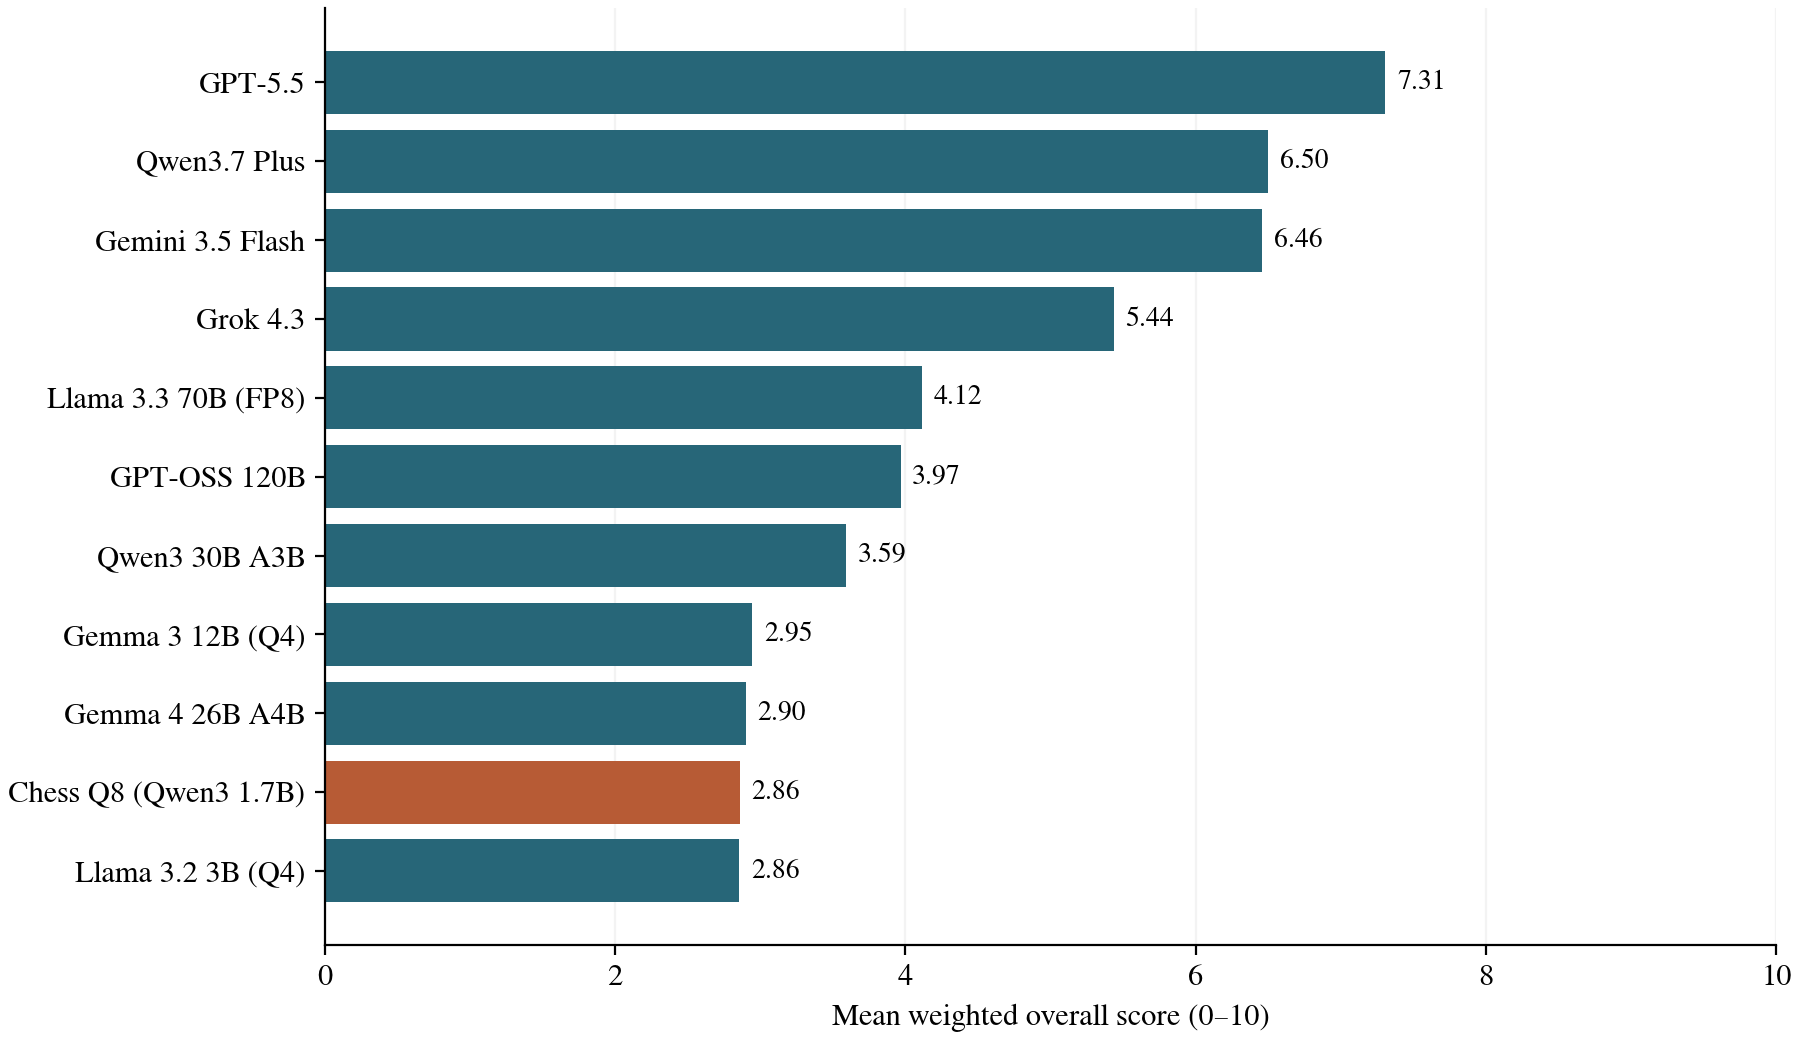
\includegraphics[width=\linewidth]{chapter3_assets/overall.png}
\caption{رتبه‌بندی میانگین امتیاز وزنی؛ داور ثابت و ۶۰ نمونه برای هر مدل}
\label{fig:overall}
\end{figure}


\subsection{جایگاه مدل کوچک در مقایسه با مدل‌های بزرگ‌تر}
شکل~\ref{fig:smallmodel} امتیاز مدل اختصاصی مبتنی بر \lr{Qwen3-1.7B} را در کنار چند مدل بزرگ‌تر نشان می‌دهد. مدل \lr{۱٫۷} میلیاردپارامتری با امتیاز \lr{۲٫۸۶} به میانگین مدل ۳ میلیاردپارامتری \lr{Llama 3.2} و دو مدل \lr{Gemma} نزدیک است. این مقایسه، مکمل رتبه‌بندی کامل ۱۱ مدل در شکل~\ref{fig:overall} است و فقط بخشی از مدل‌های آزموده‌شده را برجسته می‌کند.

\begin{figure}[htbp]
\centering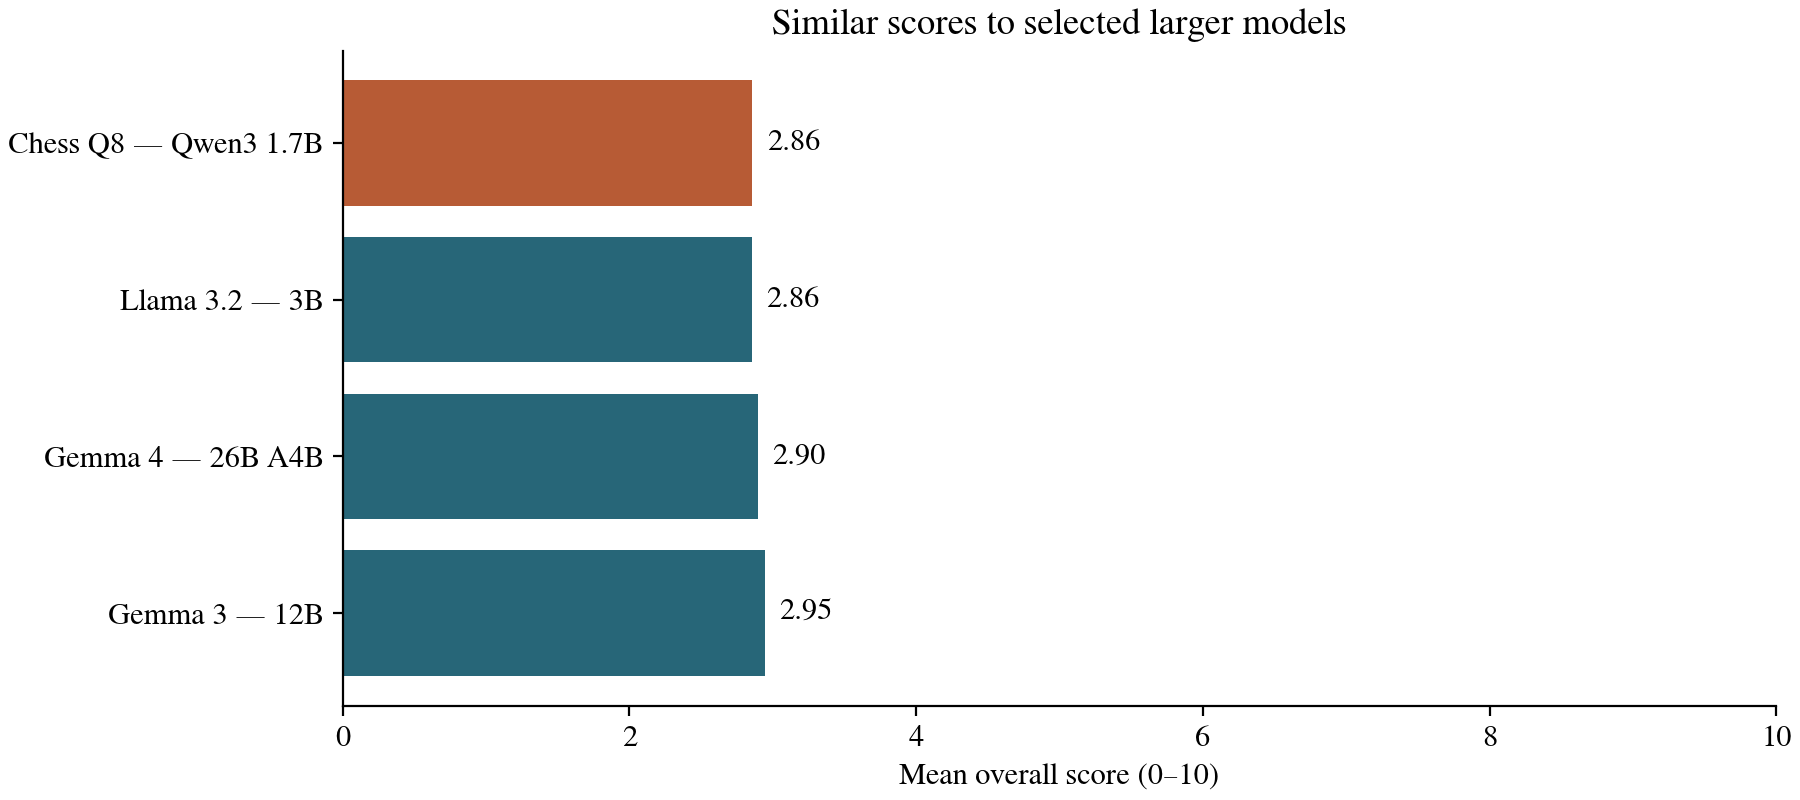
\includegraphics[width=\linewidth]{chapter3_assets/small_model_comparison.png}
\caption{مقایسه امتیاز مدل اختصاصی \lr{۱٫۷} میلیاردپارامتری با چند مدل بزرگ‌تر بر روی ۶۰ نمونه مشترک}
\label{fig:smallmodel}
\end{figure}

نزدیکی امتیاز مدل \lr{۱٫۷} میلیاردپارامتری به چند مدل با اندازه اسمی بیشتر، نتیجه‌ای امیدوارکننده برای بررسی کاربرد مدل‌های کوچک در این مسئله است. این نتیجه نشان می‌دهد که در مجموعه حاضر، اندازه بیشتر به تنهایی تضمین‌کننده امتیاز بهتر نیست. بااین‌حال، مدل‌ها از نظر آموزش، معماری، کمی‌سازی و تنظیمات اجرا یکسان نیستند؛ به‌ویژه شناسه \lr{26B A4B} به مدلی با معماری متخصص‌های ترکیبی اشاره دارد و تعداد کل پارامترها با تعداد پارامترهای فعال برابر نیست. از این مقایسه نمی‌توان نسبت مستقیم سرعت، مصرف حافظه یا هزینه را استخراج کرد. همچنین آزمون برابری آماری انجام نشده است؛ تعبیر دقیق نتیجه، «نزدیکی میانگین امتیازها در این آزمایش» است، نه برابری عمومی قابلیت مدل‌ها.

\subsection{تفاوت روانی متن و صحت محتوایی}
شکل~\ref{fig:metrics} پنج معیار را به صورت جداگانه نمایش می‌دهد. در ده مدل، میانگین روانی برابر با ۱۰ است؛ برای مدل اختصاصی نیز روانی حدود \lr{۹٫۹۷} به دست آمده است. بااین‌حال، صحت حدود \lr{۰٫۹۸}، وفاداری حدود \lr{۱٫۰۸}، مفیدبودن حدود \lr{۲٫۱۷} و پیروی از دستور حدود \lr{۸٫۱۳} هستند. پس نزدیکی امتیاز کلی به چند مدل بزرگ‌تر، نباید ضعف باقی‌مانده در معیارهای محتوایی را پنهان کند. متن می‌تواند از نظر جمله‌بندی مناسب باشد و همچنان پیام اصلی مرجع را منتقل نکند یا ادعایی ناسازگار با آن بسازد.

\begin{figure}[htbp]
\centering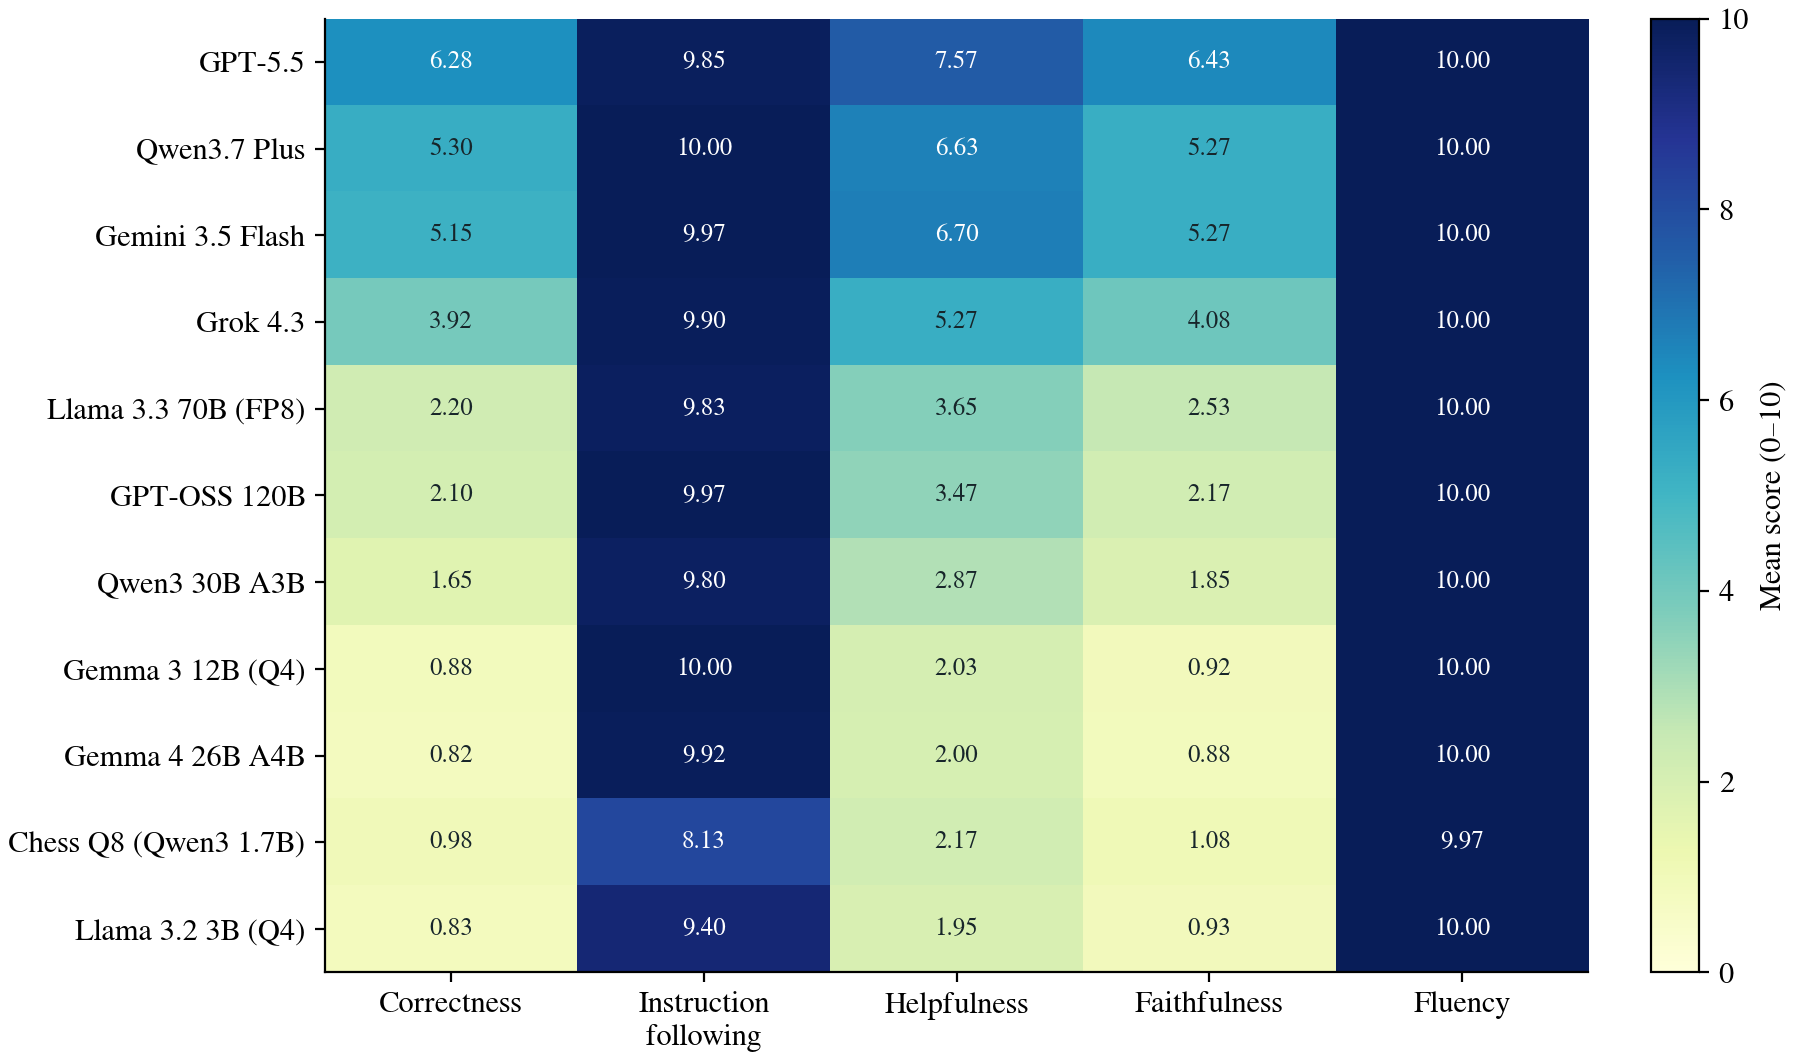
\includegraphics[width=\linewidth]{chapter3_assets/metrics.png}
\caption{میانگین پنج معیار داوری؛ رنگ تیره‌تر نشان‌دهنده امتیاز بیشتر است}
\label{fig:metrics}
\end{figure}

نزدیک بودن امتیازهای روانی به سقف مقیاس، توان تمایز این معیار را در آزمایش حاضر کاهش می‌دهد. از سوی دیگر، چون معیارهای صحت و وفاداری هر دو به مرجع وابسته‌اند، نباید آن‌ها را دو تأیید کاملاً مستقل از درستی شطرنجی فرض کرد. با این ملاحظه، نتیجه اصلی همچنان روشن است: برای انتخاب مدل آموزشی، تکیه بر خوانایی متن یا ظاهر تخصصی پاسخ کافی نیست و معیارهای محتوایی باید نقش اصلی داشته باشند.

\subsection{نتایج به تفکیک سطح نمونه‌ها}
شکل~\ref{fig:categories} امتیاز کلی را برای هر گروه نمایش می‌دهد. امتیاز \lr{GPT-5.5} در گروه‌های مبتدی، متوسط و پیشرفته به‌ترتیب \lr{۷٫۳۶}، \lr{۷٫۸۵} و \lr{۶٫۷۲} است. برای \lr{Gemini 3.5 Flash} این مقادیر \lr{۷٫۱۰}، \lr{۷٫۰۸} و \lr{۵٫۱۹} هستند. کاهش امتیاز در گروه پیشرفته برای این مدل‌ها با دشوارتر بودن انتقال مضمون برخی موقعیت‌ها سازگار است، اما به‌تنهایی رابطه علّی میان سطح بازیکن و کیفیت توضیح را اثبات نمی‌کند.

\begin{figure}[htbp]
\centering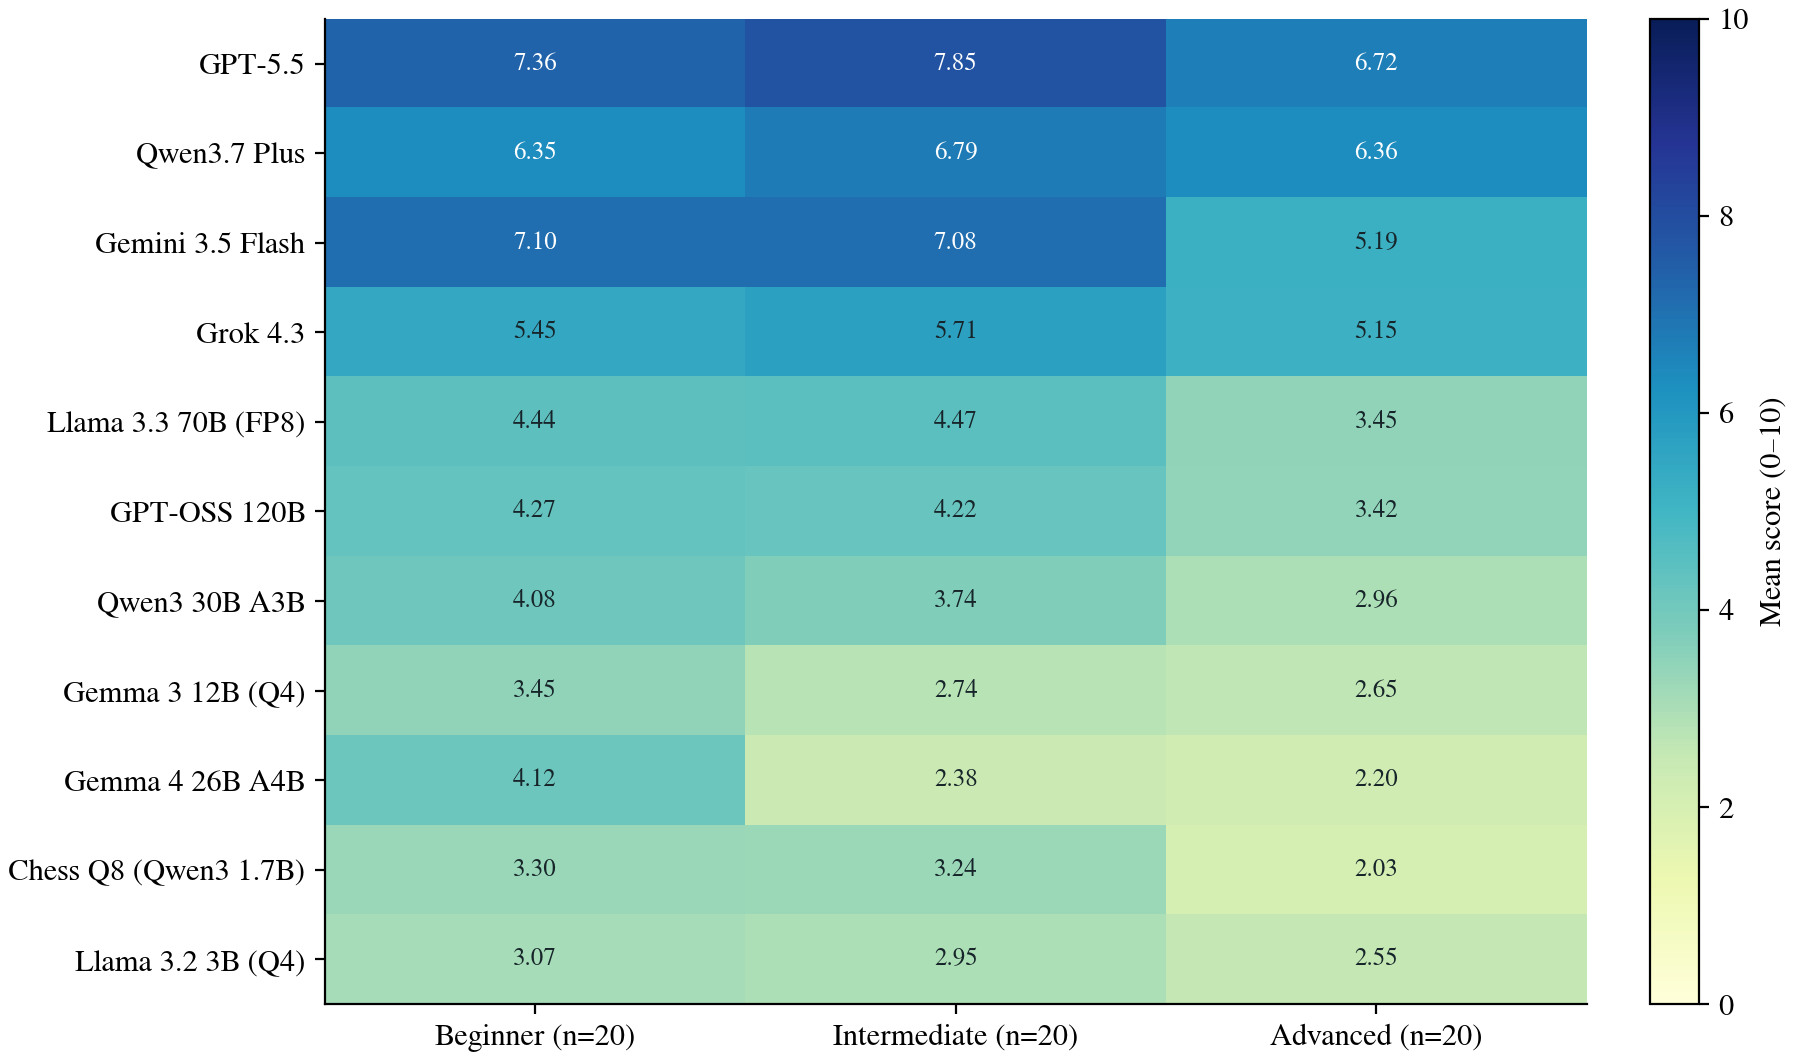
\includegraphics[width=\linewidth]{chapter3_assets/categories.png}
\caption{میانگین امتیاز کلی به تفکیک گروه؛ هر خانه حاصل ۲۰ نمونه است}
\label{fig:categories}
\end{figure}

مدل \lr{Qwen3.7 Plus} در سه گروه به‌ترتیب \lr{۶٫۳۵}، \lr{۶٫۷۹} و \lr{۶٫۳۶} امتیاز دارد و نسبت به دو مدل یادشده تغییر کمتری نشان می‌دهد. مدل اختصاصی نیز در گروه مبتدی \lr{۳٫۳۰}، متوسط \lr{۳٫۲۴} و پیشرفته \lr{۲٫۰۳} امتیاز گرفته است. این الگو نشان می‌دهد بررسی میانگین کلی به تنهایی کافی نیست؛ مدل مناسب باید علاوه بر کیفیت متوسط، در نوع موقعیت مورد استفاده نیز بررسی شود. با وجود توازن تعداد نمونه‌ها، هر گروه فقط ۲۰ نمونه دارد و تعمیم نتیجه به تمام بازی‌های آن سطح نیازمند مجموعه بزرگ‌تر است.

\subsection{بررسی یک نمونه واقعی}
شکل~\ref{fig:example} نمونه \lr{g1\_m38} از گروه پیشرفته را نشان می‌دهد. حرکت ثبت‌شده \lr{Bxf8} است و تصویر، موقعیت قبل و بعد از گرفتن رخ با فیل سفید را نمایش می‌دهد. توضیح مرجع بر این نکته تأکید دارد که ارزش ظاهری گرفتن رخ نباید پیامد تاکتیکی ادامه بازی را پنهان کند: پاسخ حریف تهدیدی علیه وزیر ایجاد می‌کند و دنباله تعویض‌ها می‌تواند به زیان سفید تمام شود. این توصیف، خلاصه پیام مرجع ذخیره‌شده است، نه تحلیل تازه‌ای که جداگانه توسط موتور تأیید شده باشد.

\begin{figure}[htbp]
\centering
\includegraphics[width=\linewidth]{../../artifacts/analysis_images/g1_m38__model_chess-q8_0.png}
\caption{نمونه واقعی گروه پیشرفته؛ وضعیت قبل در چپ و وضعیت بعد در راست}
\label{fig:example}
\end{figure}

پاسخ مدل اختصاصی در همین نمونه، به حرکت‌های دیگری مانند \lr{Nxe4} و \lr{Nxc3} اشاره کرده و پیامد حرکت را با حمله به شاه و کنترل صفحه توضیح داده است. این پاسخ با درس اصلی مرجع هم‌راستا نیست. داور برای صحت، وفاداری و مفیدبودن آن امتیاز صفر و برای روانی و پیروی از دستور امتیاز ده ثبت کرده است؛ حاصل وزنی برابر با \lr{۲٫۰۰} است. این نمونه به صورت عینی نشان می‌دهد که امتیاز خوب زبانی می‌تواند در کنار خطای محتوایی شدید قرار بگیرد و امتیاز پیروی از دستور نیز رعایت همه جزئیات الگوی تولید را تضمین نمی‌کند.

\section{محدودیت‌ها و پیشنهادهای بهبود}
نخستین محدودیت، اندازه مجموعه آزمون است. شصت موقعیت برای مقایسه اولیه و یافتن الگوهای خطا مفید است، اما پوشش کامل گشایش، وسط‌بازی، آخر‌بازی و انواع تاکتیک‌ها را تضمین نمی‌کند. همچنین نمونه‌های برخاسته از یک بازی ممکن است مستقل از یکدیگر نباشند. توسعه مجموعه با بازی‌های متنوع‌تر، ثبت منشأ هر نمونه و جداسازی در سطح بازی، اعتبار ارزیابی آینده را افزایش می‌دهد.

دومین محدودیت به داوری مربوط است. امتیازها حاصل قضاوت یک مدل بر اساس یک توضیح مرجع هستند. مرجع ممکن است کامل نباشد و توضیح درست دیگری را پوشش ندهد؛ داور نیز ممکن است خطا کند یا به سبک نوشتار حساس باشد. نامزد خانواده \lr{Gemma} نیز در میان مدل‌ها وجود دارد و اثر احتمالی هم‌خانواده بودن با داور در این آزمایش جداگانه سنجیده نشده است. افزودن ارزیابی انسانی توسط بازیکنان خبره و بررسی ادعاهای متن با ابزار شطرنج می‌تواند این محدودیت را کاهش دهد.

سومین محدودیت، نبود مقایسه کنترل‌شده برای سهم اجزای روش است. برای سنجش پایداری نتیجه، تکرار آزمایش با تنظیمات یکسان و نمونه‌های متنوع‌تر لازم است. آزمایش حاضر نشان نمی‌دهد که افزودن ویژگی‌ها، تغییر الگوی ورودی، تنظیم دقیق یا تغییر دقت کمی‌سازی به تنهایی چه اثری دارد. برای پاسخ به این پرسش‌ها باید یک مدل ثابت را با و بدون هر مؤلفه، روی نمونه‌های یکسان ارزیابی کرد. همچنین آزمایش مدل پایه و نسخه تنظیم‌شده آن با شرایط یکسان برای سنجش اثر آموزش دامنه ضروری است.

برای بهبود تولید توضیح، تهیه جفت‌های آموزشی موقعیت و توضیح صحیح، محدود کردن پاسخ به ادعاهای قابل پشتیبانی و بررسی خروجی پیش از نمایش به کاربر پیشنهاد می‌شود. در مواردی که مدل پاسخ معتبر نمی‌دهد یا شواهد کافی در دسترس نیست، سامانه می‌تواند از ارائه توضیح قطعی خودداری کند و خطای تولید را آشکار گزارش دهد. این راهکارها پیشنهاد ادامه کار هستند و در نتایج فعلی به عنوان قابلیت آزموده‌شده محسوب نمی‌شوند.

در نهایت، برای ادعای کارآمدی محاسباتی باید زمان پاسخ، مصرف حافظه، مشخصات سخت‌افزار و هزینه اجرای مدل‌ها به طور مستقل اندازه‌گیری شوند. امکان اجرای محلی یک دستاورد اجرایی است، اما جایگزین سنجش کمی سرعت و منابع نیست. به همین ترتیب، برتری عددی در این مجموعه به معنای بهبود قطعی یادگیری کاربران نیست و سنجش اثر آموزشی به مطالعه کاربری نیاز دارد.

\section{جمع‌بندی و نتیجه‌گیری}
در این پروژه، یک مسیر نرم‌افزاری برای ترکیب تحلیل موتور شطرنج، ویژگی‌های موقعیت و تولید زبان طبیعی پیاده‌سازی شد. همچنین مجموعه آزمونی متوازن با ۶۰ نمونه و فرایندی مشترک برای ذخیره، تطبیق و ارزیابی پاسخ ۱۱ مدل فراهم گردید. بدین ترتیب، هدف ایجاد محیطی قابل بررسی برای تولید و مقایسه توضیحات شطرنجی تحقق یافته است.

نتیجه مهم آزمایش آن است که مدل اختصاصی مبتنی بر \lr{Qwen3-1.7B}، با وجود داشتن تنها \lr{۱٫۷} میلیارد پارامتر، به امتیاز \lr{۲٫۸۶} از ده رسید؛ این امتیاز تقریباً برابر با \lr{Llama 3.2 3B} و نزدیک به \lr{Gemma 4 26B A4B} و \lr{Gemma 3 12B} است. بنابراین، در این مجموعه محدود، مدل کوچک توانسته است از نظر میانگین امتیاز به چند مدل بزرگ‌تر نزدیک شود. این یافته، همراه با امکان اجرای محلی، انگیزه‌ای برای ادامه توسعه و ارزیابی مدل‌های سبک در تولید توضیح شطرنجی فراهم می‌کند.

این مقایسه اثر مستقل آموزش دامنه را اثبات نمی‌کند. همچنین صحت \lr{۰٫۹۸} و وفاداری \lr{۱٫۰۸} در برابر روانی \lr{۹٫۹۷} نشان می‌دهند که توضیح روان هنوز تضمین‌کننده تحلیل درست نیست. بهترین مدل این آزمایش امتیاز \lr{۷٫۳۱} دارد؛ پس نتیجه حاضر، هم‌سطح بودن عمومی مدل کوچک با همه مدل‌های بزرگ یا آمادگی آن برای ارائه توضیح بدون نظارت را نشان نمی‌دهد.

دستاورد پروژه، ایجاد سامانه قابل اجرا و نشان دادن ظرفیت مدل کوچک در مقایسه با چند مدل بزرگ‌تر است. ادامه کار باید بر داده آموزشی جفت‌شده با موقعیت، کنترل ادعاهای متن با شواهد صفحه، مقایسه مدل پایه و نسخه آموزش‌دیده، ارزیابی انسانی و سنجش مستقل زمان و منابع متمرکز شود. این مسیر می‌تواند نزدیکی امتیازهای مشاهده‌شده را به توضیح آموزشی دقیق‌تر و قابل اعتمادتر تبدیل کند.
